

% microtype: Tipografía.
% mathpazo: Usa la fuente Palatino.
\documentclass[a4paper, 11pt]{article}
\usepackage[protrusion=true,expansion=true]{microtype}
\usepackage{mathpazo}
\usepackage{booktabs}
\usepackage{multicol}
\usepackage{multirow}

% Indentación de párrafos para Palatino
\setlength{\parindent}{0pt}
  \parskip=8pt
\linespread{1.05} % Change line spacing here, Palatino benefits from a slight increase by default


%%% Castellano.
% noquoting: Permite uso de comillas no españolas.
% lcroman: Permite la enumeración con numerales romanos en minúscula.
% fontenc: Usa la fuente completa para que pueda copiarse correctamente del pdf.
\usepackage[spanish,es-noquoting,es-lcroman]{babel}
\usepackage[utf8]{inputenc}
\usepackage[T1]{fontenc}
\selectlanguage{spanish}


%%% Gráficos
\usepackage{graphicx} % Required for including pictures
\usepackage{wrapfig} % Allows in-line images
\usepackage[usenames,dvipsnames]{color} % Coloring code


%%% Matemáticas
\usepackage{amsmath}
\usepackage{hyperref}
%%% Código


\usepackage{listings}
\usepackage{graphicx}



%%% Bibliografía
\makeatletter
\renewcommand\@biblabel[1]{\textbf{#1.}} % Change the square brackets for each bibliography item from '[1]' to '1.'
\renewcommand{\@listI}{\itemsep=0pt} % Reduce the space between items in the itemize and enumerate environments and the bibliography



%----------------------------------------------------------------------------------------
%	TÍTULO
%----------------------------------------------------------------------------------------
% Configuraciones para el título.
% El título no debe editarse aquí.
\renewcommand{\maketitle}{
  \begin{flushright} % Right align
  
  {\LARGE\@title} % Increase the font size of the title
  
  \vspace{50pt} % Some vertical space between the title and author name
  
  {\large\@author} % Author name
  \\\@date % Date
  \vspace{40pt} % Some vertical space between the author block and abstract
  \end{flushright}
}

%% Título
\title{\textbf{Memoria de la práctica 1}\\ % Title
Algorítmica} % Subtitle

\author{\textsc{Fco. Javier Sáez Maldonado}\\ % Author
\textsc{Laura Gómez Garrido}\\
\textsc{Luis Antonio Ortega Andrés}\\
\textsc{Pedro Bonilla Nadal}\\
\textsc{Daniel Pozo Escalona}\vspace{2cm}
\\{\textit{Universidad de Granada}}} % Institution

\date{\today} % Date



%----------------------------------------------------------------------------------------
%	DOCUMENTO
%----------------------------------------------------------------------------------------

\begin{document}

\maketitle % Print the title section


%% Índice
{\parskip=2pt
  \tableofcontents
}
\pagebreak

%%% Inicio del documento


\section*{Introducción}

En esta primera práctica, vamos a estudiar la eficiencia tanto empírica como teórica de ciertos algoritmos. Para ello, realizaremos pruebas empíricas con nuestros propios equipos para comprobar que la eficiencia se ajusta a la que calculada de forma teórica.

Comenzaremos presentando los algoritmos que vamos a estudiar. Son algoritmos bastante conocidos, así como sus eficiencias teóricas. Estos son:
\begin{enumerate}
	\item Algoritmo de ordenación \textbf{burbuja}.
	\item Algoritmo de ordenación por \textbf{inserción}.
	\item Algoritmo de ordenación por \textbf{selección}.
	\item Algoritmo de ordenación \textbf{mergesort}, basado en la técnica divide y vencerás.
	\item Algoritmo de ordenación \textbf{quicksort}.
	\item Algoritmo de ordenación \textbf{heapsort}.
	\item Algoritmo de \textbf{Floyd}.
	\item Algoritmo de \textbf{Hanoi}.
\end{enumerate}

Los ejecutaremos en varias máquinas, a saber:
\begin{enumerate}    
	\item Máquina A: Procesador Intel Core I7-5700HQ, 6M Cache y 3.5 Ghz.
	\item Máquina B: Procesador Intel Core I7-4712MQ , 6M cache y 2.30Ghz
	\item Máquina C: Procesador: Intel Core i7-4510U ,2.00GHz
	\item Máquina D: Máquina Virtual VirtualBox versión 5.1.112r112440(Qt5.6.2) dentro de una Máquina C.

\end{enumerate}

\section{Cálculo de la eficiencia empírica}
A fin de facilitar el cálculo de la eficiencia empírica, escribimos un guion que automatizase el proceso de realizar las ejecuciones pedidas para cada algoritmo, recoger los datos y organizarlos en carpetas. %El código es el siguiente:

%\begin{lstlisting}
%mkdir resultados ejecutable 2> /dev/null

%for i in *.cpp
%do
%    j=`echo $i | cut -f 1 -d .`
%    g++ -O2 $i -o ../ejecutable/$j

%    echo $j

%	      echo "" > ../resultados/$j.dat
%	      k="1"
%	      while [ $k -le 28 ]
%	      do
%	          ../ejecutable/$j $k >> ../resultados/$j.dat
%	          k=$[$k+1]
%	      done
%done

%\end{lstlisting}
Además, según el tipo de algoritmo, hemos ido variando el número de veces que se ejecuta el código.
 %El que hemos mostrado es el que ejecuta el programa de Hanoi. 
En la siguiente tabla se muestra el tamaño de los datos de entrada en cada iteración, para cada algoritmo.

\begin{tabular}{lllll}
	Orden de eficiencia & Algoritmo & Tamaño inicial & Incremento & Tamaño final\\ \midrule
	\multirow{3}{*}{$O(n\log n)$} & \textit{Heapsort} & \multirow{3}{*}{1000} & \multirow{3}{*}{1000} & \multirow{3}{*}{100000} \\
	& \textit{Mergesort} & & &\\
	& \textit{Quicksort} & & &\\ \midrule
	\multirow{3}{*}{$O\left(n^2\right)$} & Burbuja & \multirow{3}{*}{500} & \multirow{3}{*}{500} & \multirow{3}{*}{50000} \\
	& Inserción & & &\\
	& Selección & & &\\ \midrule
	$O\left(n^3\right)$ & Floyd & 25 & 25 & 2500 \\\midrule
	$O\left(2^n\right)$ & Hanoi & 1 & 1 & 28
	
\end{tabular}

\subsection{Tablas de las ejecuciones}
A continuación se presentan los datos resultantes de ejecutar los distintos algoritmos, agrupados por clases de eficiencia. Escribiremos  las tablas generadas por el computador de tipo $A$, si bien incompletas, para no ocupar todo el documento con ellas. Estas tablas podrán ser consultadas en una carpeta incluída en el proyecto.

\subsubsection{ Tabla algoritmos $O(n^2)$}
\begin{tabular}{@{}llll@{}}
\toprule
Tamaño Vector & Burbuja  & Inserción & Selección  \\ \midrule
500           & 0.000183 & 0.00012   & 9.41e-05   \\
1000          & 0.000676 & 0.00041   & 0.00033464 \\
1500          & 0.001421 & 0.000889  & 0.00073601 \\
2000          & 0.002645 & 0.001483  & 0.00124963 \\
2500          & 0.004357 & 0.002291  & 0.002069   \\
3000          & 0.00658  & 0.003276  & 0.002789   \\
3500          & 0.009617 & 0.004485  & 0.003708   \\
4000          & 0.013066 & 0.005808  & 0.00491    \\
4500          & 0.017328 & 0.007279  & 0.006437   \\
5000          & 0.022303 & 0.00898   & 0.007507   \\
5500          & 0.0279   & 0.010837  & 0.008995   \\
6000          & 0.034061 & 0.012819  & 0.010721   \\
6500          & 0.041173 & 0.01515   & 0.012625   \\
7000          & 0.049032 & 0.017688  & 0.014594   \\
7500          & 0.057096 & 0.020175  & 0.017596   \\
8000          & 0.06641  & 0.023064  & 0.018863   \\
8500          & 0.076047 & 0.026317  & 0.02148    \\
9000          & 0.087017 & 0.029131  & 0.023866   \\
9500          & 0.099032 & 0.032499  & 0.026604   \\
10000         & 0.11069  & 0.03597   & 0.029735   \\
10500         & 0.123762 & 0.039592  & 0.032609   \\
11000         & 0.138682 & 0.043482  & 0.03555    \\
11500         & 0.151532 & 0.047382  & 0.038855   \\
12000         & 0.166319 & 0.051606  & 0.042199   \\
12500         & 0.181765 & 0.055837  & 0.045834   \\
13000         & 0.198691 & 0.060376  & 0.049303   \\
13500         & 0.21569  & 0.064976  & 0.053129   \\
14000         & 0.231813 & 0.069198  & 0.057271   \\
14500         & 0.250401 & 0.074645  & 0.061438   \\
%%%%%%%%%%%%%%%%%%%%%%%%%%%%%%%%%%%%%%%%%%%%%

15000         & 0.269076 & 0.079654  & 0.065577   \\
15500         & 0.290561 & 0.084977  & 0.069896   \\
16000         & 0.31048  & 0.090637  & 0.07443    \\
16500         & 0.330982 & 0.0963    & 0.07922    \\
17000         & 0.353309 & 0.103345  & 0.084177   \\
17500         & 0.373751 & 0.109385  & 0.09186    \\
18000         & 0.397518 & 0.115501  & 0.094513   \\
18500         & 0.426722 & 0.122327  & 0.099572   \\
19000         & 0.4511   & 0.129006  & 0.104891   \\
%19500         & 0.473987 & 0.136012  & 0.11034    \\
%20000         & 0.499128 & 0.143031  & 0.116565   \\
\bottomrule
\end{tabular}

\subsubsection{Tablas de algoritmos $n^3$}

\begin{tabular}{@{}llll@{}}
\toprule
Tamaño Vector & Mergesort   & Heapsort & Quicksort \\ \midrule
1000          & 4.1423e-05  & 6.1e-05  & 4.9e-05   \\
2000          & 9.9989e-05  & 0.000142 & 9.7e-05   \\
3000          & 0.000187499 & 0.000223 & 0.00016   \\
4000          & 0.000221424 & 0.000268 & 0.000192  \\
5000          & 0.000303942 & 0.000367 & 0.000286  \\
6000          & 0.000399219 & 0.000416 & 0.000285  \\
7000          & 0.00039881  & 0.000476 & 0.000372  \\
8000          & 0.000474348 & 0.00052  & 0.00038   \\
9000          & 0.000563394 & 0.000629 & 0.000425  \\
10000         & 0.000649712 & 0.000784 & 0.000484  \\
11000         & 0.000845    & 0.000783 & 0.000528  \\
12000         & 0.000895    & 0.000903 & 0.000607  \\
13000         & 0.000838    & 0.000944 & 0.000659  \\
14000         & 0.000898    & 0.001027 & 0.000732  \\
15000         & 0.000968    & 0.001096 & 0.000847  \\
16000         & 0.001065    & 0.001107 & 0.000836  \\
17000         & 0.00123     & 0.001167 & 0.000906  \\
18000         & 0.001332    & 0.001311 & 0.001203  \\
19000         & 0.001334    & 0.001318 & 0.000972  \\
20000         & 0.001487    & 0.001464 & 0.00107   \\
21000         & 0.001621    & 0.00148  & 0.001146  \\
22000         & 0.001656    & 0.001573 & 0.001186  \\
23000         & 0.001772    & 0.00167  & 0.001244  \\
24000         & 0.001905    & 0.001867 & 0.001324  \\
25000         & 0.002049    & 0.00199  & 0.001348  \\
26000         & 0.001807    & 0.001893 & 0.001459  \\
27000         & 0.001879    & 0.00198  & 0.00151   \\
28000         & 0.001937    & 0.002086 & 0.001498  \\
29000         & 0.002007    & 0.00212  & 0.001579  \\
30000         & 0.002077    & 0.002397 & 0.001664  \\
31000         & 0.002285    & 0.002336 & 0.001741  \\
32000         & 0.002266    & 0.002378 & 0.001808  \\
33000         & 0.00244     & 0.002577 & 0.001808  \\
34000         & 0.002571    & 0.002529 & 0.00185   \\
35000         & 0.002595    & 0.002641 & 0.001948  \\
36000         & 0.002639    & 0.002733 & 0.002045  \\
37000         & 0.002763    & 0.002752 & 0.002108  \\
38000         & 0.002913    & 0.002832 & 0.002109  \\ \bottomrule
%39000         & 0.002961    & 0.002919 & 0.002195  \\
%40000         & 0.003039    & 0.003069 & 0.002246  \\\bottomrule
\end{tabular}


\subsubsection{Tabla algoritmo Hanoi}


\begin{tabular}{@{}ll@{}}
\toprule
Tamaño Vector & Hanoi    \\ \midrule
1             & 1,00E-06 \\
2             & 1,00E-06 \\
3             & 1,00E-06 \\
4             & 1,00E-06 \\
5             & 1,00E-06 \\
6             & 1,00E-06 \\
7             & 1,00E-06 \\
8             & 2,00E-06 \\
9             & 2,00E-06 \\
10            & 4,00E-06 \\
11            & 6,00E-06 \\
12            & 1.1e-05  \\
13            & 1.8e-05  \\
14            & 3.8e-05  \\
15            & 8.2e-05  \\
16            & 0.000174 \\
17            & 0.000324 \\
18            & 0.000663 \\
19            & 0.001226 \\
20            & 0.002177 \\
21            & 0.004413 \\
22            & 0.008785 \\
23            & 0.017613 \\
24            & 0.034917 \\
25            & 0.069979 \\
26            & 0.138508 \\
27            & 0.276828 \\
28            & 0.552919 \\ \bottomrule
\end{tabular}
\subsubsection{Tabla algoritmo Floyd}
\begin{tabular}{@{}ll@{}}
\toprule
Tamaño Vector & Floyd    \\ \midrule
50            & 0.000147 \\
75            & 0.000422 \\
100           & 0.000841 \\
125           & 0.001555 \\
150           & 0.002624 \\
175           & 0.004146 \\
200           & 0.005986 \\
225           & 0.008689 \\
250           & 0.011423 \\
275           & 0.015214 \\
300           & 0.019555 \\
325           & 0.024801 \\
350           & 0.030623 \\
375           & 0.037862 \\
400           & 0.045488 \\
425           & 0.058492 \\
450           & 0.069071 \\
475           & 0.079011 \\
500           & 0.08839  \\
525           & 0.102404 \\
550           & 0.119307 \\
575           & 0.134324 \\
600           & 0.161119 \\
625           & 0.172804 \\
650           & 0.192393 \\
675           & 0.216992 \\
700           & 0.240593 \\
725           & 0.269456 \\
750           & 0.295816 \\
775           & 0.327231 \\
800           & 0.359917 \\
825           & 0.408639 \\
850           & 0.433239 \\
875           & 0.47942  \\
900           & 0.522784 \\
925           & 0.577851 \\
950           & 0.618519 \\
975           & 0.675189 \\
1000          & 0.759402 \\ \bottomrule
\end{tabular}

\section{Realización de las gráficas.}
Para la realización de las gráficas usamos, sobre los datos previamente ofrecidos, el programa veusz (\hyperref[github]{https://github.com/jeremysanders/veusz} |hyperref[pagina oficial]{http://home.gna.org/veusz/}). En  ellas hemos buscado la máxima claridad y legibilidad de estas.

\subsection{Gráfica de algoritmos $O(n\log n)$}
  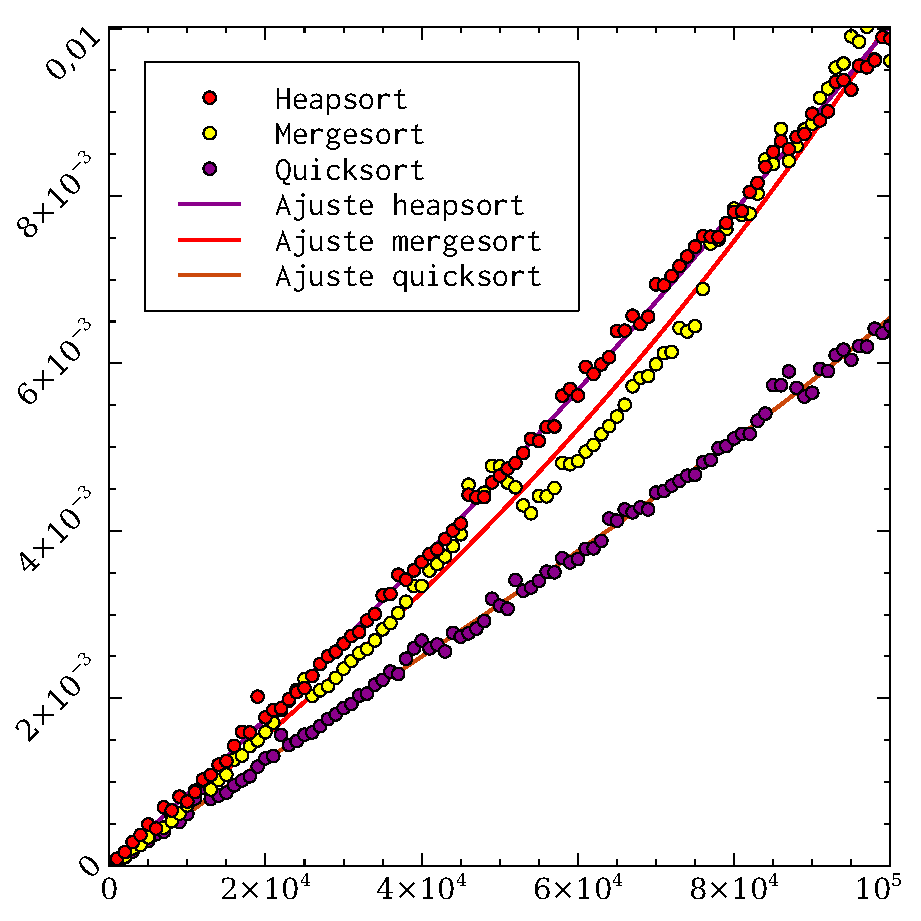
\includegraphics[]{nlogn_ajuste.eps}

\subsection{Gráfica de algoritmos $O(n^2)$}
  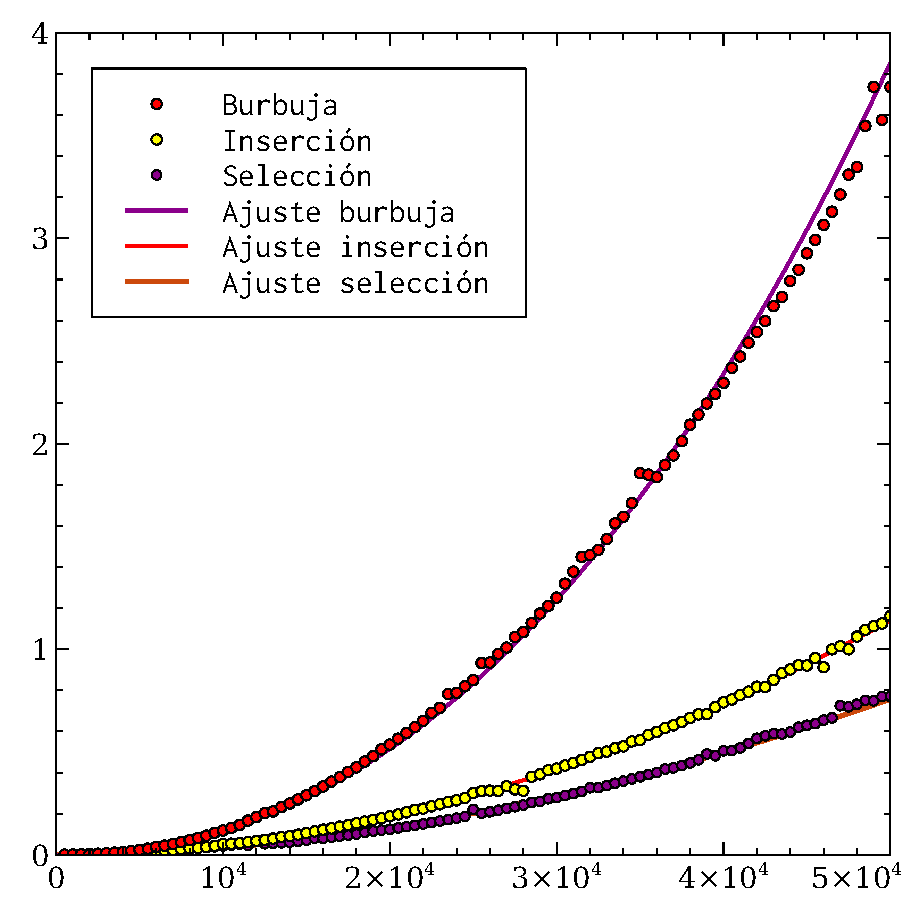
\includegraphics[]{n2_ajuste}
\subsection{Gráfica del algoritmo $O(n^3)$}
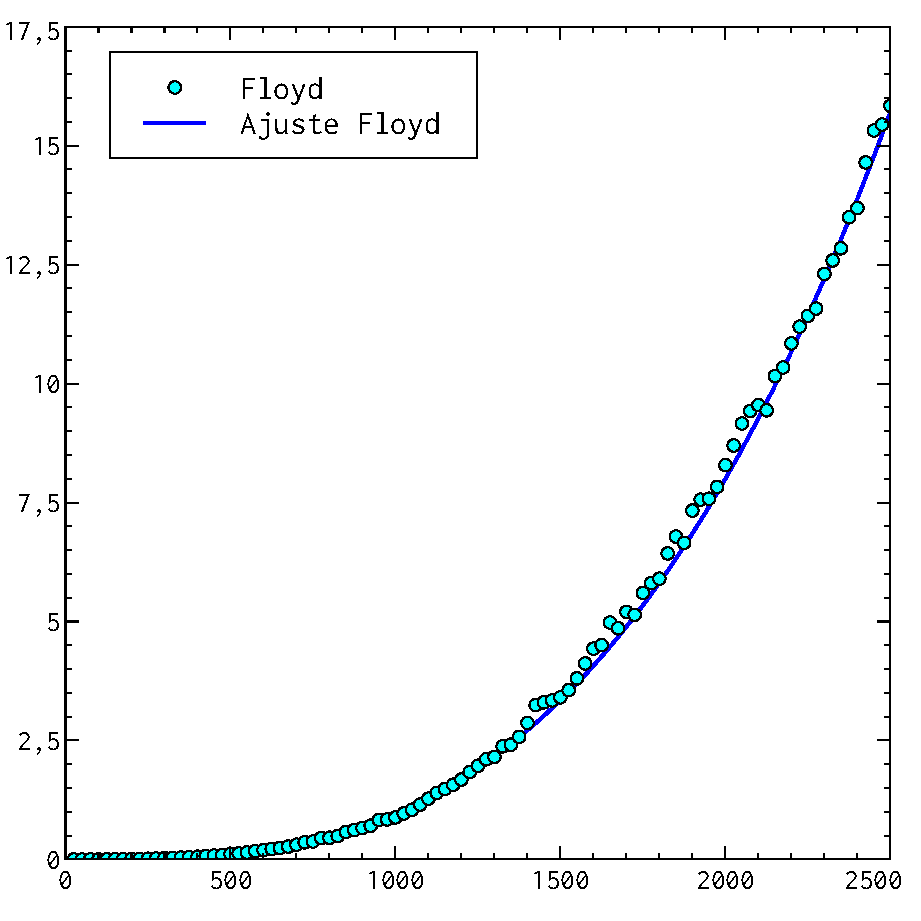
\includegraphics[]{n3_ajuste.eps}
\subsection{Gráfica del algoritmo $O(2^n)$}
 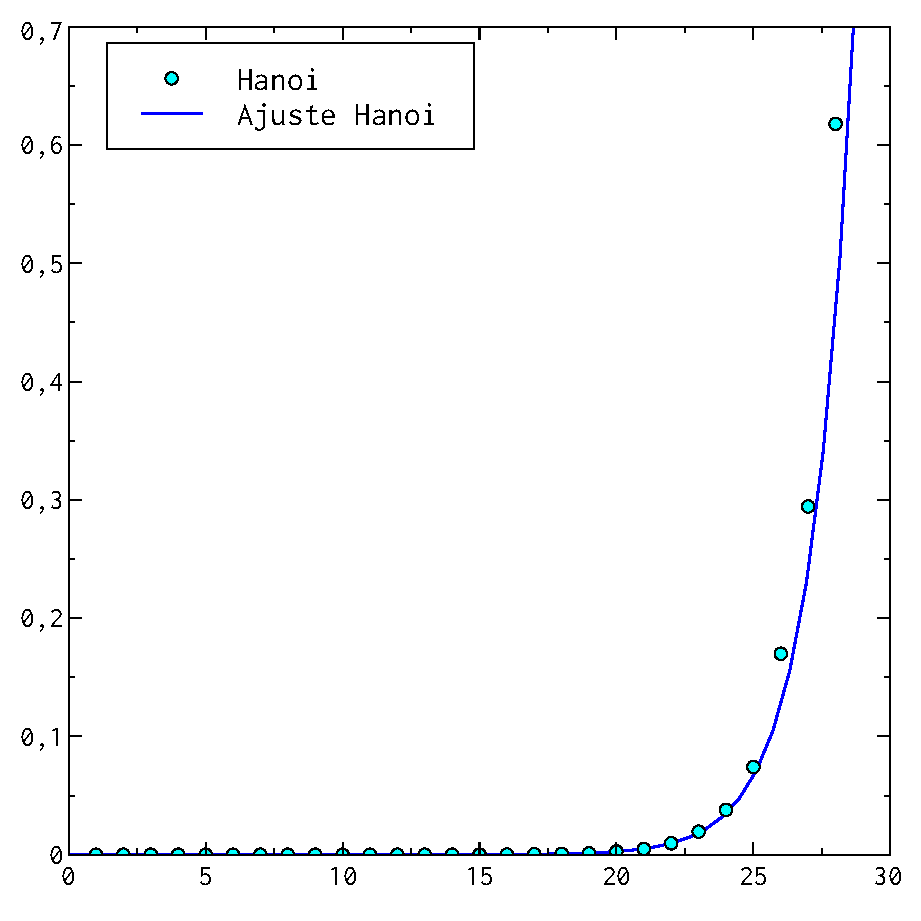
\includegraphics[]{2n_ajuste.eps}
 
 
 
 
\section{Cálculo de la eficiencia híbrida}
A continuación calcularemos la eficiencia híbrida de los datos de la máquina B, para ello utilizaremos el mismo programa que hemos utlizado para elaborar las gráficas, indicándole qué tipo de ajuste queremos que nos realice para cada algoritmo. Para los algoritmos de eficiencia logaritmica, le indicamos que la curva a partir de la cual queremos que parametrice es  $ax\log(x)+bx$ y dándonos los siguientes resultados:
\begin{center}
\begin{tabular}{ll}
  Algoritmo & Coeficientes\\ \hline\noalign{\smallskip}
  \textit{Heapsort} & $\begin{array}{ll}
  a = 4,45661980236212e-9\\
b = 4,57091330896553e-8
\end{array}$ \\\hline\noalign{\smallskip}
  \textit{Mergesort} & $\begin{array}{ll}
  a = 1,04427553800116e-8\\
b = -2,58720994439492e-8
\end{array}$\\\hline\noalign{\smallskip}
  \textit{Quicksort} & $\begin{array}{ll}
  a = 2,79493370281663e-9\\
b = 3,29731080614046e-8
\end{array}$\\ \hline\noalign{\smallskip}
  
\end{tabular}
\end{center}
De la misma forma, para los algoritmos eficiencia cuadrática, le hemos indicado que la curva sobre la cual queremos que ajuste se trata de $a+bx+cx^2$ y obteniendo así:
\begin{center}
\begin{tabular}{ll}
Algoritmo & Coeficientes\\ \hline\noalign{\smallskip}
Burbuja  &  $\begin{array}{lll}
  a = 0,00082695543722856\\
b = -1,78008100621617e-6\\
c = 1,41949043281942e-9
\end{array}$  \\\hline\noalign{\smallskip}
  Inserción  & $\begin{array}{lll}
  a = 9,34565785754161e-6\\
b = 4,03176585100252e-8\\
c = 4,60339062991612e-10
\end{array}$\\\hline\noalign{\smallskip}
  Selección  & $\begin{array}{lll}
  a = -3,46794858274209e-5\\
b = 1,18720037408458e-7\\
c = 3,13826775410318e-10
\end{array}$\\
\end{tabular}
\end{center}

Ahora, nos encontramos con Floyd cuya eficiencia es cúbica y tendríamos pues que ajustar sobre la curva $a+bx+cx^2+dx^3$ y obteniendo de esta forma que:
\begin{center}
\begin{tabular}{ll}
Algoritmo & Coeficientes\\ \hline\noalign{\smallskip}
Floyd  & $\begin{array}{llll}
  a = -0,0001373576928425\\
b = 7,19449328754654e-6\\
c = -6,0356967827879e-8\\
d = 1,02809541531643e-9
\end{array}$\\
\end{tabular}
\end{center}

Finalmente, sólo nos queda ver qué ocurre con Hanoi cuya curva es $a2^{bx}$ y nos da:
\begin{center}
\begin{tabular}{ll}
Algoritmo & Coeficientes\\ \hline\noalign{\smallskip}
Hanoi  & $\begin{array}{ll}
  a = 7,0670287742651e-9\\
b = 0,92649353651508
\end{array}$
\end{tabular}
\end{center}

\section{Ejercicio 4}
Otro aspecto interesante a analizar mediante este tipo de estudio es la variación de la eficiencia empírica en función de parámetros externos tales como: las opciones de compilación utilizada (con/sin optimización), el ordenador donde se realizan las pruebas, el sistema operativo, etc. Sugiera algún estudio de este tipo, consulte con el profesor de prácticas y llévelo a cabo.

Para llevar a cabo la resolución de este ejercicio, utilizando el script de realización de las tablas, lo que hemos hecho ha sido realizar las ejecuciones en las distintas máquinas y exponerlas en una misma gráfica para ver las diferencias que se obtienen de los distintos procesadores y prestaciones, con los mismos algoritmos. Las gráficas que se generan están hechos con los datos que estarán en las tablas que expondremos en un fichero externo a la memoria. Pasamos a exponer las gráficas.

\begin{enumerate}
  \item Burbuja:\\
  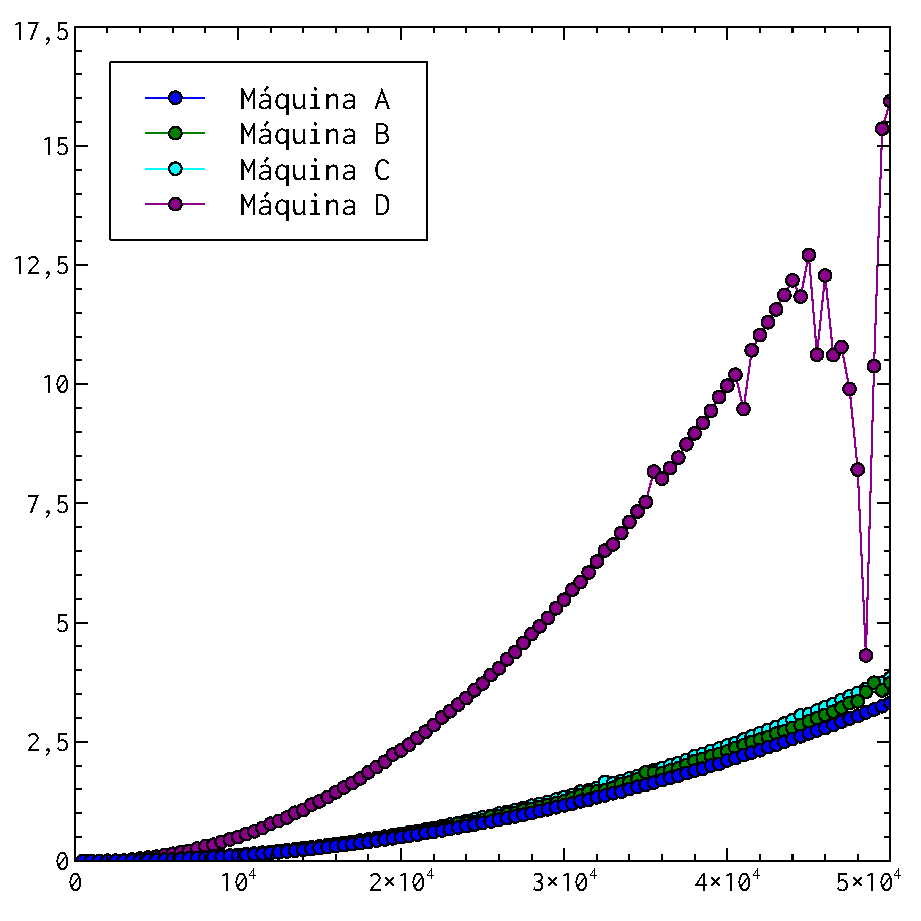
\includegraphics[scale=0.5]{burbuja_todos.eps}\\
  Podemos observar que las máquinas de prestaciones similares tienen tiempos similares en este pesado algoritmo, y que la máquina D(la máquina virtual) comienza pronto a realizar las ejecuciones mucho más despacio que las demás y luego, por razones de procesamiento, consigue en una ejecución acercarse al tiempo normal de ejecución pero luego vuelve a su estado de procesamiento lento.
  \item Inserción:\\
  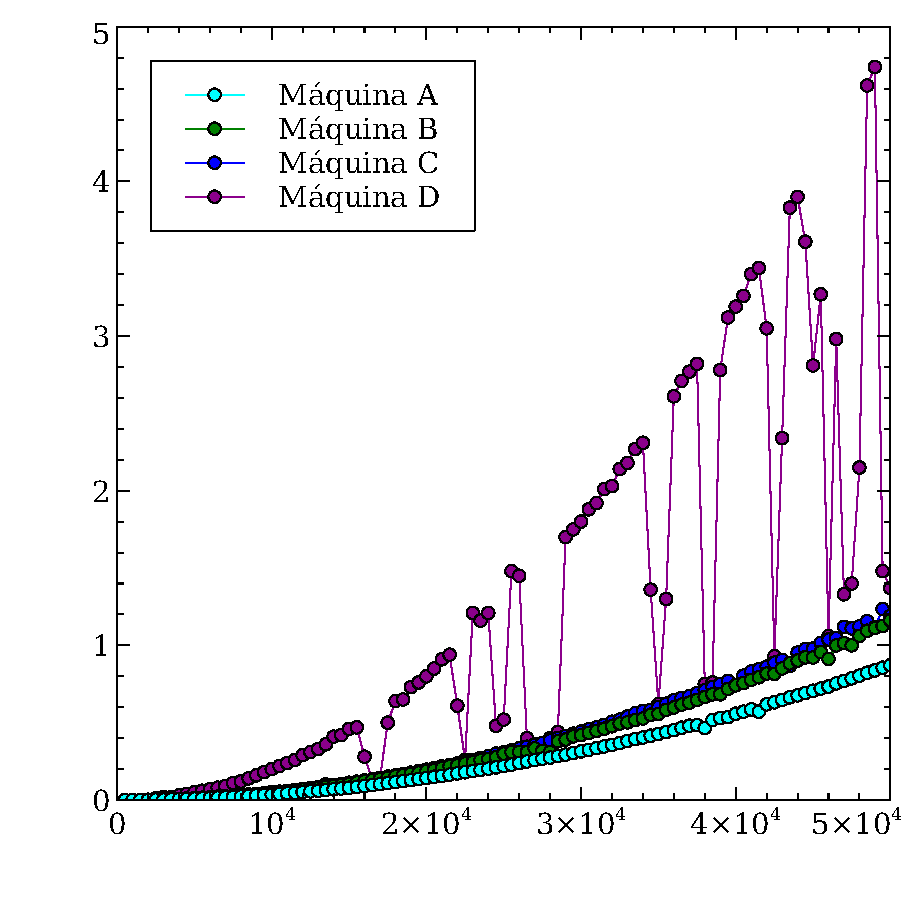
\includegraphics[scale=0.5]{insercion_todos.eps}\\
  Podemos ver que nuestra máquina con mejor procesador realiza las ejecuciones de este algoritmo mejor que las demás, alejándose al aumentar el tamaño de las demás. Además, también tenemos un comportamiento extraño en la máquina D, que a veces hace ejecuciones muy lentas y otras veces realiza ejecuciones con velocidad similar a las máquinas B y C.
  \item Selección:\\
  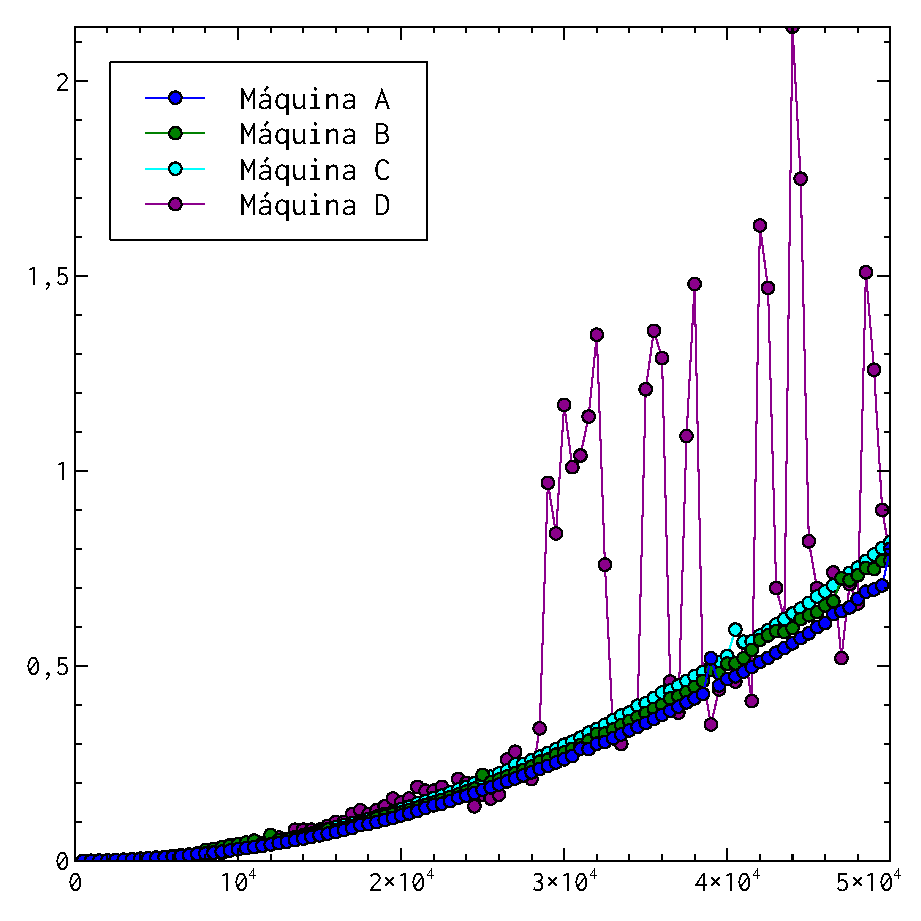
\includegraphics[scale=0.5]{seleccion_todos.eps}\\
  En este algoritmo, todas las máquinas comienzan tardando lo mismo hasta la mitad del tamaño de las ejecuciones, lo cual es sorprendente por parte de la máquina D, pero luego se aleja mucho realizando grandes oscilaciones en los tiempos de ejecución.
  \item Heapsort:\\
  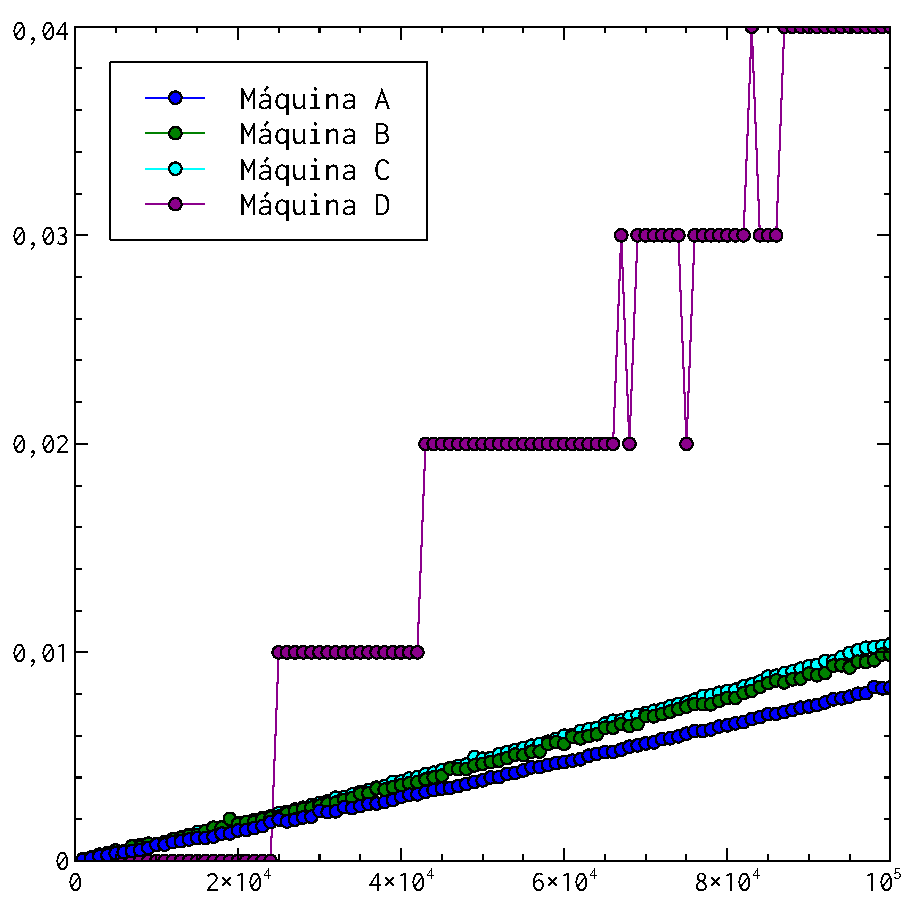
\includegraphics[scale=0.5]{heapsort_todos.eps}\\
  En el algoritmo Heapsort, podemos observar un comportamiento un tanto peculiar de la máquina virtual. Como se puede observar, comienza con los tiempos en cero, por lo que probablemente la máquina no pudo ejecutar el algoritmo y luego se ve como va ascendiendo en escalones, tardando exactamente el mismo tiempo para varios tamaños del vector, lo cual no tiene mucho sentido. Las demás máquinas sí que realizan un comportamiento normal. Es importante denotar que este error es producido por la máquina, ya que todas las máquinas utilizan el mismo script para realizar las ejecuciones.
  \item Mergesort:\\
  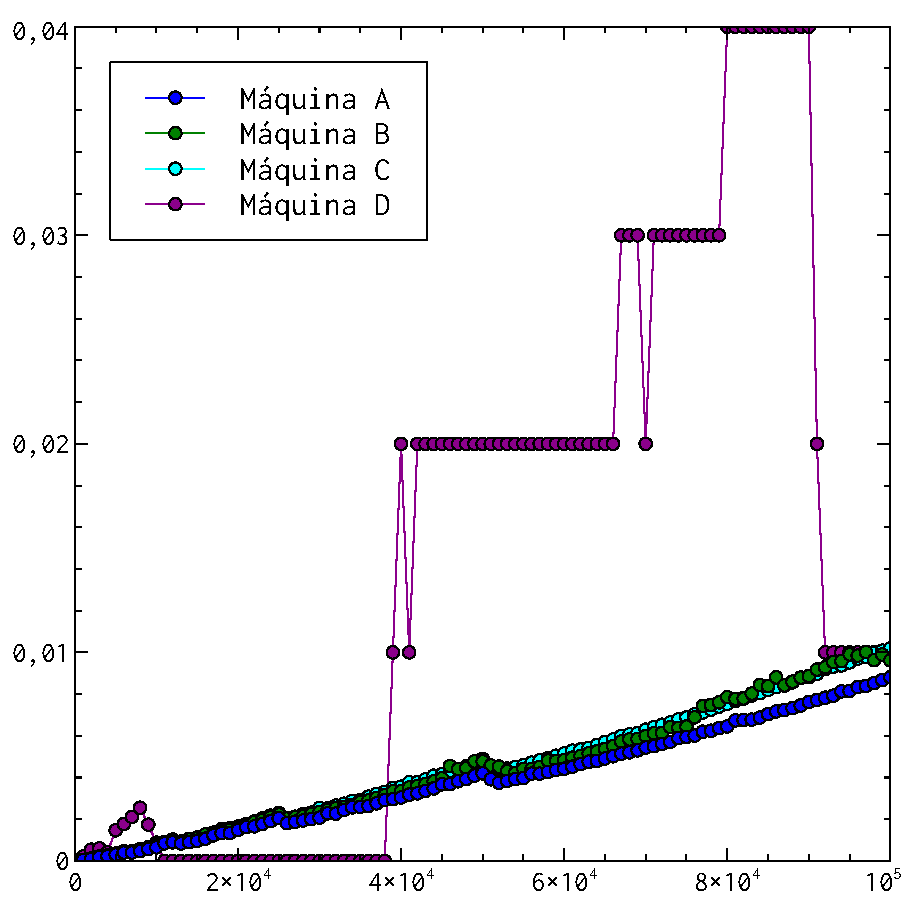
\includegraphics[scale=0.5]{mergesort_todos.eps}\\
  En Mergesort, de nuevo la máquina virtual da un comportamiento extraño, empieza ejecutando bien(aunque lento) el algoritmo, luego hasta $4x10^4$ no puede ejecutar el algoritmo y por último realiza las ejecuciones con tiempos, como en el anterior algoritmo, que ascienden en escalón. Por otro lado, también es notable el comportamiento de las máquinas A,B y C, que llevan un ritmo bastante similar durante toda la ejecución.
  \item Quicksort:\\
  \includegraphics[scale=0.5]{quicksort_todos.eps}\\
  En este algoritmo, las tres máquinas principales llevan un ritmo bastante similar y la máquina virtual se separa mucho de ellas desde el principio, teniendo un comportamiento similar al que tiene en los algoritmos anteriores.
  \item Hanoi:\\
  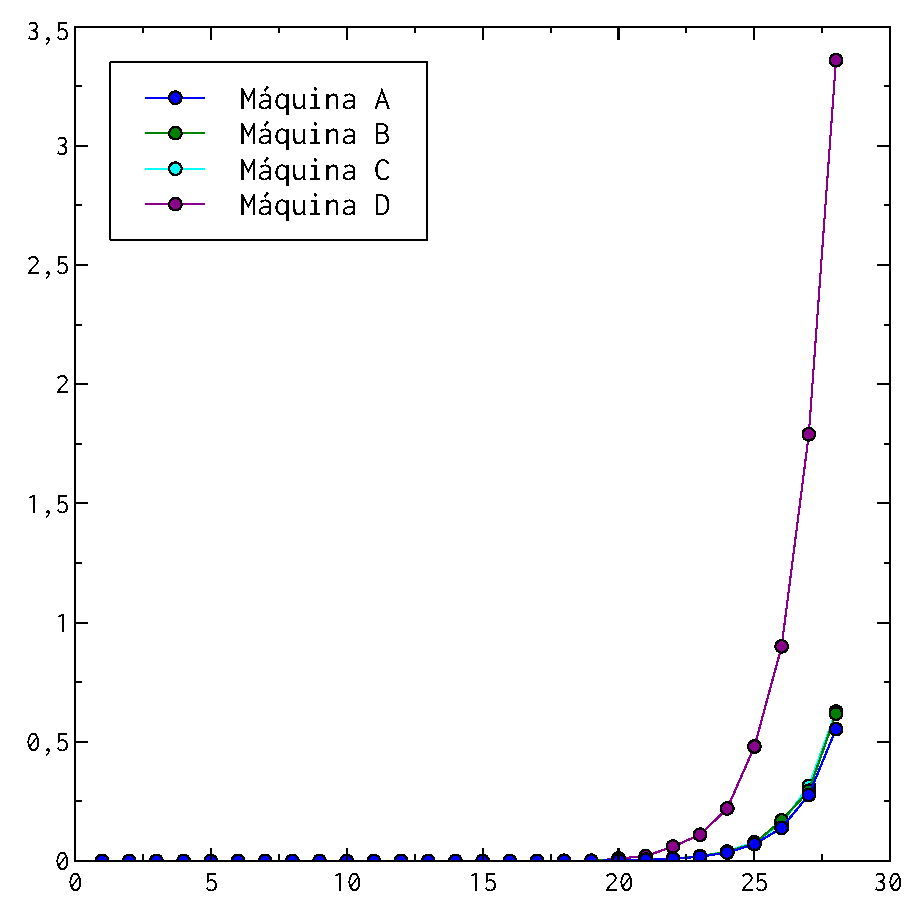
\includegraphics[scale=0.5]{hanoi_todos.eps}\\
  En este caso, volvemos a la normalidad con la máquina $D$, aunque podemos notarle que aunque las tres máquinas reales vayan al mismo ritmo, la máquina virtual se separa antes de ellas para comenzar a realizar la curva ascendente.
  \item Floyd:\\
  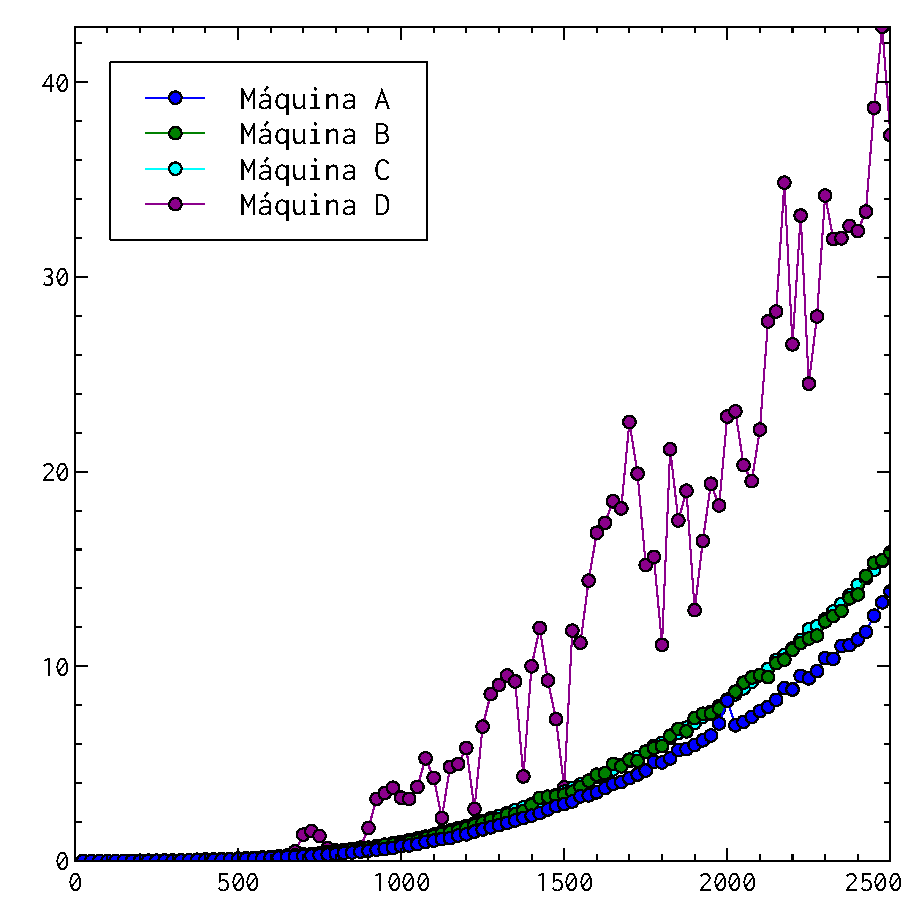
\includegraphics[scale=0.5]{floyd_todos.eps}\\

  En el último algoritmo a analizar, podemos ver que la máquina virtual se separa rápidamente d elas demás en cuanto a tiempo de ejecución y que en torno al tamaño $2000$ del vector, la máquina $A$ también se separa del resto de máquinas y tarda menos en el tiempo de ejecución
  \subsection{Conclusiones}
  Como conclusión a este ejercicio, podemos afirmar que las tres máquinas reales ($A,B$ y $C$) tienen comportamientos muy similares en las ejecuciones aunque, por lo general, la máquina $A$ consigue sacar ventaja en tiempo a las otras dos debido a su ventaja en características de procesamiento. Por otro lado, también se observa fácilmente que en la mayoría de los algoritmos, la máquina virtual genera tiempos muy dispares a los de las demás máquinas.
\end{enumerate}
\end{document}
